\documentclass[a4paper,11pt]{article}
\usepackage[utf8]{inputenc}
\usepackage{graphicx}
\usepackage{enumerate}
\usepackage{geometry}
\usepackage{fancyhdr}
\usepackage{minted}
\usepackage{xcolor}
\usepackage[colorlinks = true,
            linkcolor = blue,
            urlcolor  = blue,
            citecolor = blue]{hyperref}

\geometry{total={210mm,297mm},
left=25mm,right=25mm,%
bindingoffset=0mm, top=20mm,bottom=20mm}

\graphicspath{ {./images/} }

\renewcommand*\sfdefault{phv}
\renewcommand\familydefault{\sfdefault}

% \renewcommand{\thesubsubsection}{\thesubsection.\alph{subsubsection}}

% \newmintedfile{html}{
%     linenos,
%     breaklines,
%     python3,
%     numbersep=8pt,
%     frame=single,
%     framesep=3mm} 

\newcommand*{\TitleFont}{%
      \usefont{\encodingdefault}{\rmdefault}{b}{n}%
      \fontsize{16}{20}%
      \selectfont}

\linespread{1.3}

% my own titles
\makeatletter
\renewcommand{\maketitle}{
\begin{center}
\vspace{2ex}
{\huge \textsc{\@title}}
\vspace{1ex}
\\
\rule{\linewidth}{0.5pt}\\
\@author \hfill \@date
\vspace{4ex}
\end{center}
}
\makeatother

\definecolor{bg}{rgb}{0.95,0.95,0.95}


% custom footers and headers
\pagestyle{fancy}
\lhead{}
\chead{}
\rhead{}
\lfoot{Assignment 2 : Regular expression/ text processing tools/ autotools }
\cfoot{}
\rfoot{Page \thepage}
\renewcommand{\headrulewidth}{0pt}
\renewcommand{\footrulewidth}{0pt}
%%----------%%%----------%%%----------%%%----------%%%

\begin{document}

\newminted{bash}{fontsize=\scriptsize, 
    linenos,
    breaklines,
    numbersep=8pt,
    frame=single,
    bgcolor=bg,
    framesep=3mm} 

\newminted{makefile}{fontsize=\scriptsize, 
    linenos,
    breaklines,
    numbersep=8pt,
    frame=single,
    bgcolor=bg,
    framesep=3mm} 



% \newminted{all}{linenos, frame=single}

% \usemintedstyle{monokai}
\usemintedstyle{manni}
% \usemintedstyle{xcode}
% \usemintedstyle{vs}
% \usemintedstyle{autumn}
% \usemintedstyle{colorful}
% \usemintedstyle{trac}


\title{ \TitleFont Assignment 2 : Regular expression/ text processing tools/ autotools }

\author{Emil Sharifulllin, Innopolis University}

\date{\today}

\maketitle

\tableofcontents

\section{Assignment 1}

\subsection{Debian packaging system}
The main Debian package management tool is \textbf{dpkg}. Dpkg is a program that allows users to install remove and configure packages. dpkg needs *.deb files which is special archives, containing binary executables, configuration files, man/info pages, copyright information, and other documentation. Debian systems also contain \textbf{apt}-Advanced Packaging Tool is a high-level tool that uses dpkg under itself. APT have repositories of .deb packages and there is not need to download .deb files manually.

\subsubsection{How does it work?}
dpkg checks package for dependencies and if system doesn't contain certain dependency dpkg stops installation with error. Then it extracts files from .deb file, run preistall scripts, move binaries to system folder, run postinstall script. Last step is to add record to it's own registry, that in this system installed certain package. \hl{dpkg have two kinds of packages: binary and source. Both is an ar archives with data. Binary packages is a .deb files which usually contains executable files, libraries, and documentation associated with this certain package. Source packages usually contains .orig.tar.gz file with sources and .diff.gz file with debian-specific changes.}\\\\
apt is a tool that can automatically download .deb file, download dependencies .deb files. Then apt install package using dpkg.

\subsubsection{How does it deal with dependencies?}
\hl{Every debian package can be dependent on other packages. This dependencies listed in \textbf{control} file. Control file contains information about package name, version, author, architecture and dependencies. Here you can see example of control file:}

\begin{bashcode}
Package: hello
Version: 2.9-2+deb8u1
Architecture: amd64
Maintainer: Santiago Vila <sanvila@debian.org>
Installed-Size: 145
Depends: libc6 (>= 2.14)
Conflicts: hello-traditional
Breaks: hello-debhelper (<< 2.9)
Replaces: hello-debhelper (<< 2.9), hello-traditional
Section: devel
Priority: optional
Homepage: http://www.gnu.org/software/hello/
Description: example package based on GNU hello
  The GNU hello program produces a familiar, friendly greeting.  It
  allows non-programmers to use a classic computer science tool which
  would otherwise be unavailable to them.
  .
  Seriously, though: this is an example of how to do a Debian package.
  It is the Debian version of the GNU Project's `hello world' program
  (which is itself an example for the GNU Project).
\end{bashcode}

dpkg cannot install missing dependencies if dependency is not installed on system dpkg fails with installation. apt downloads and installs dependencies before install package. dpkg supports following types of dependencies:

\begin{itemize}
  \item \textbf{A depends on B} B must be installed in order for A to function
  \item \textbf{A recommends B} A will work without B, but some useful functionality won’t be available
\item \textbf{A suggests B} a weaker version of recommends, that is, A is “nice to have” together with B
\item \textbf{A conflicts with B} A and B cannot exist on the same system
\item \textbf{A replaces B} B files will be overwritten by A’s files
\item \textbf{A breaks B} A will render B unusable
\item \textbf{A provides B} all functions of B are supplied by A
\item \textbf{A enhances B} reverse variant of suggests
\end{itemize}

\subsubsection{Does it use the GNU build tools? How? If not what does it use?}
In general dpkg don't use build tools to install package because packages spreads as a .deb files which contains already built binaries. But dpkg uses build tools to create deb files for example in dpkg-buildpackage script. \hl{dpkg also uses debian build tools to build and install package from sources. The autors of source package can add additional information about packages using to build theirs package from sources. This information is called build-dependencies.}

\subsection{Open SUSE packaging system}

Open SUSE system contains RPM and zypper package systems. RPM is very similar to dpkg and works with compiled binary executables. RPM can install, deinstall and update packages. zypper is similar to apt and contain repository and can automative download and install packages.

\subsubsection{How does it work?}
RPM works with .rpm files which is binary files and contains following data:

\begin{itemize}
  \item The lead, which identifies the file as an RPM file and contains some obsolete headers.
  \item The signature, which can be used to ensure integrity and/or authenticity.
  \item The header, which contains metadata including package name, version, architecture, file list, etc.
  \item A file archive (the payload), which usually is in cpio format, compressed with gzip. The rpm2cpio tool enables retrieval of the cpio file without needing to install the RPM package.
\end{itemize}

To create new rpm package usually uses SPEC file. This is special recipe file that contain data about package and steps to compile package. 

\subsubsection{How does it deal with dependencies?}
RPM does not care about dependencies. To handle dependencies you should use high level package managers for example zypper or YaST. Zypper have own repository so it can download dependent packages from it and preinstall it.
\subsubsection{Does it use the GNU build tools? How?}
As a dpkg RPM works with pre-builded binary packages and build tools is used during cretion of package.

% \begin{pythoncode}
% main():
%     print("hello, world")
%     return 0
% \end{pythoncode}

\section{Assignment 2}
\subsection{Look for a small and simple game on the web}
For this assignment I chose \href{https://github.com/JohnAnthony/TROG}{TROG} game: 
\subsubsection{Download its source package for Ubuntu}
Source code for TROG game can be fuod at \href{https://github.com/JohnAnthony/TROG.git}{https://github.com/JohnAnthony/TROG.git} git repository.

\subsubsection{Create a binary from the source for the desktop}
To create binary and install game on my system I heed to make following commands:

\begin{bashcode}
$ git clone https://github.com/JohnAnthony/TROG.git
$ cd TROG
$ sudo apt install ncurses-dev -y
$ make
$ sudo make install
\end{bashcode}

My system by default not contain ncurses library so I need to install it manually.

\subsubsection{Read about cross-compilation and try to create a binary from the source for the i386 architecture. Try and install that on your experimentation computer.}
Game that I downloaded didn't have configure script. So to compile it on my system I needed to change Makefile.

\begin{makefilecode}
CFLAGS+= -std=c++0x -Wall -pedantic -O0 -ggdb -Iinclude -m32 
OBJECTS= spell.o trog.o level.o game.o character.o enemy.o geometry.o tile.o \
item.o gui.o potion.o scrollable_menu.o treasure.o stattome.o equippable.o \
debug.o enemy_type.o
LIBS= -lncurses
CXX ?= g++

trog: ${OBJECTS}
        ${CXX} ${CFLAGS} -o $@ ${OBJECTS} ${LIBS}

#Objects with a header file
%.o: src/%.cpp include/*.hpp
        ${CXX} ${CFLAGS} -c -o $@ $<

clean:
        -rm -f $(OBJECTS) trog

install: trog
        cp -v trog /usr/bin/

.PHONY: clean
\end{makefilecode}

In this file I added -m32 option to CFLAGS variable.\\
To allow gcc compile this code in crosscompile mode I installed following libraries.
\begin{bashcode}
$ sudo apt install gcc-multilib g++-multilib -y
$ sudo apt install lib32ncurses5-dev -y
\end{bashcode}

After it I make following:

\begin{bashcode}
$ make clear
$ make
$ file trog                             
trog: ELF 32-bit LSB executable, Intel 80386, version 1 (SYSV), dynamically linked, interpreter /lib/ld-linux.so.2, for GNU/Linux 2.6.32, BuildID[sha1]=b413be74881edbcd7c1ff3f3b9fb294d15f8610e, not stripped
\end{bashcode}

Final result:\\

\includegraphics[width=17cm]{1.png}
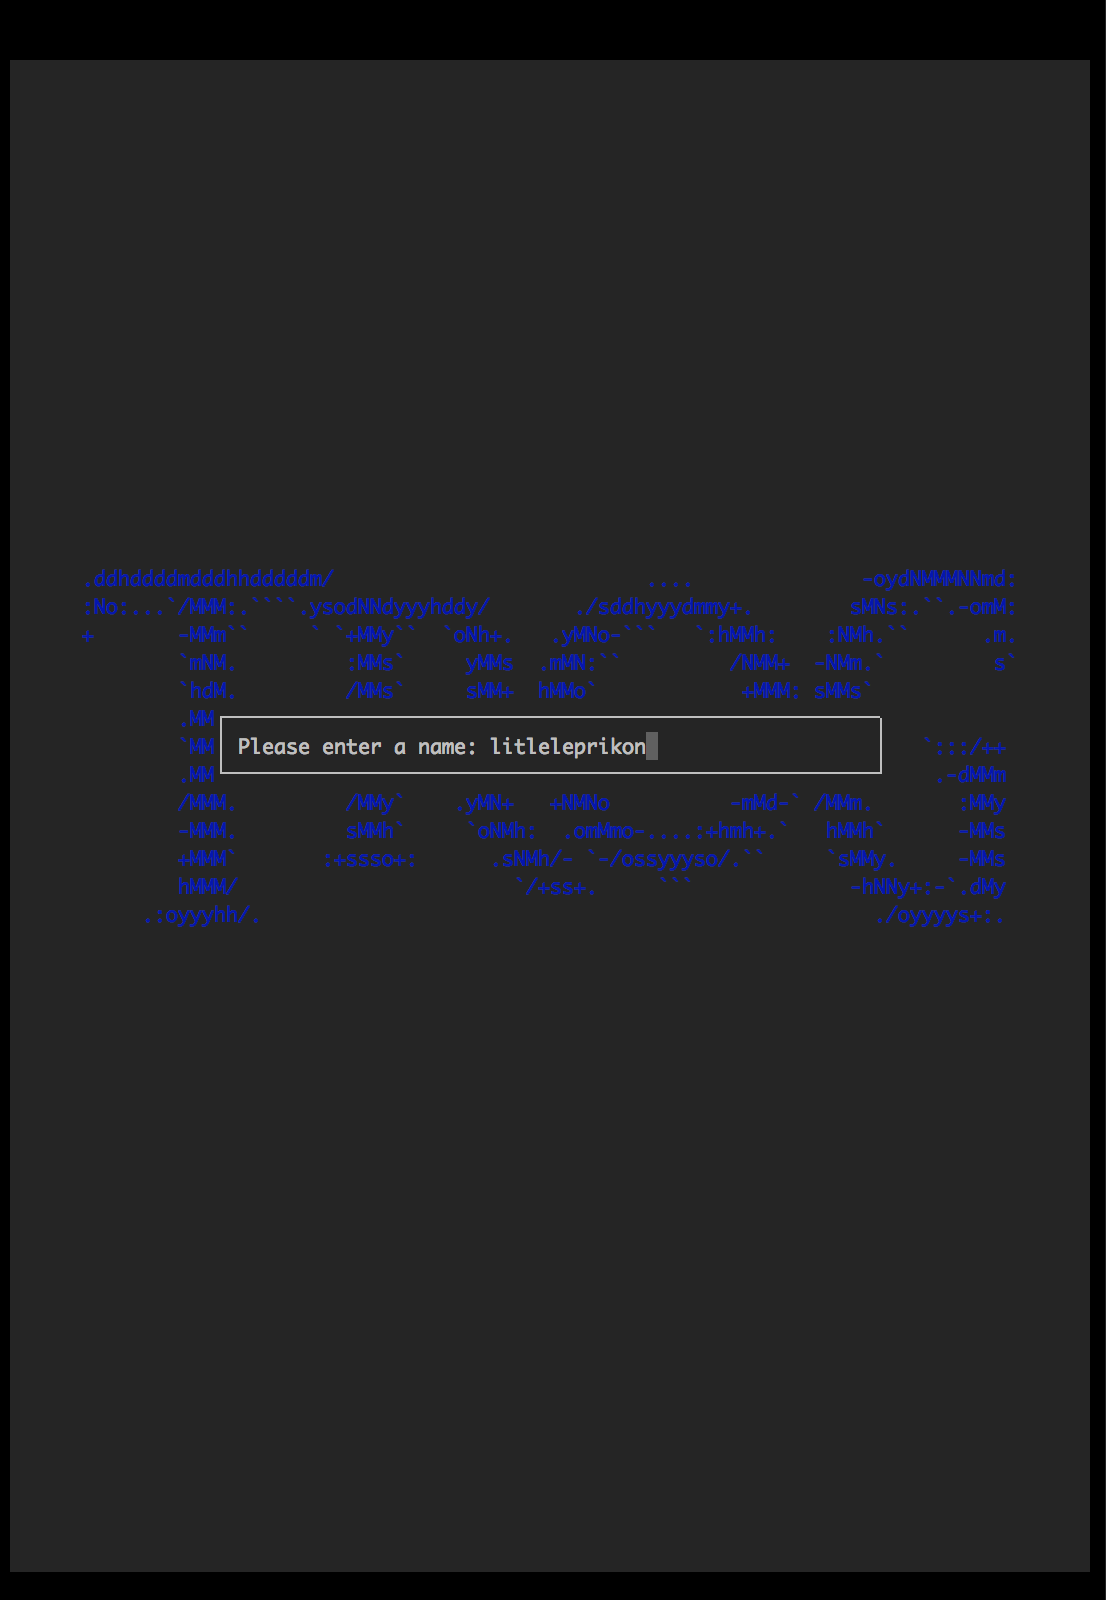
\includegraphics[width=17cm]{2.png}
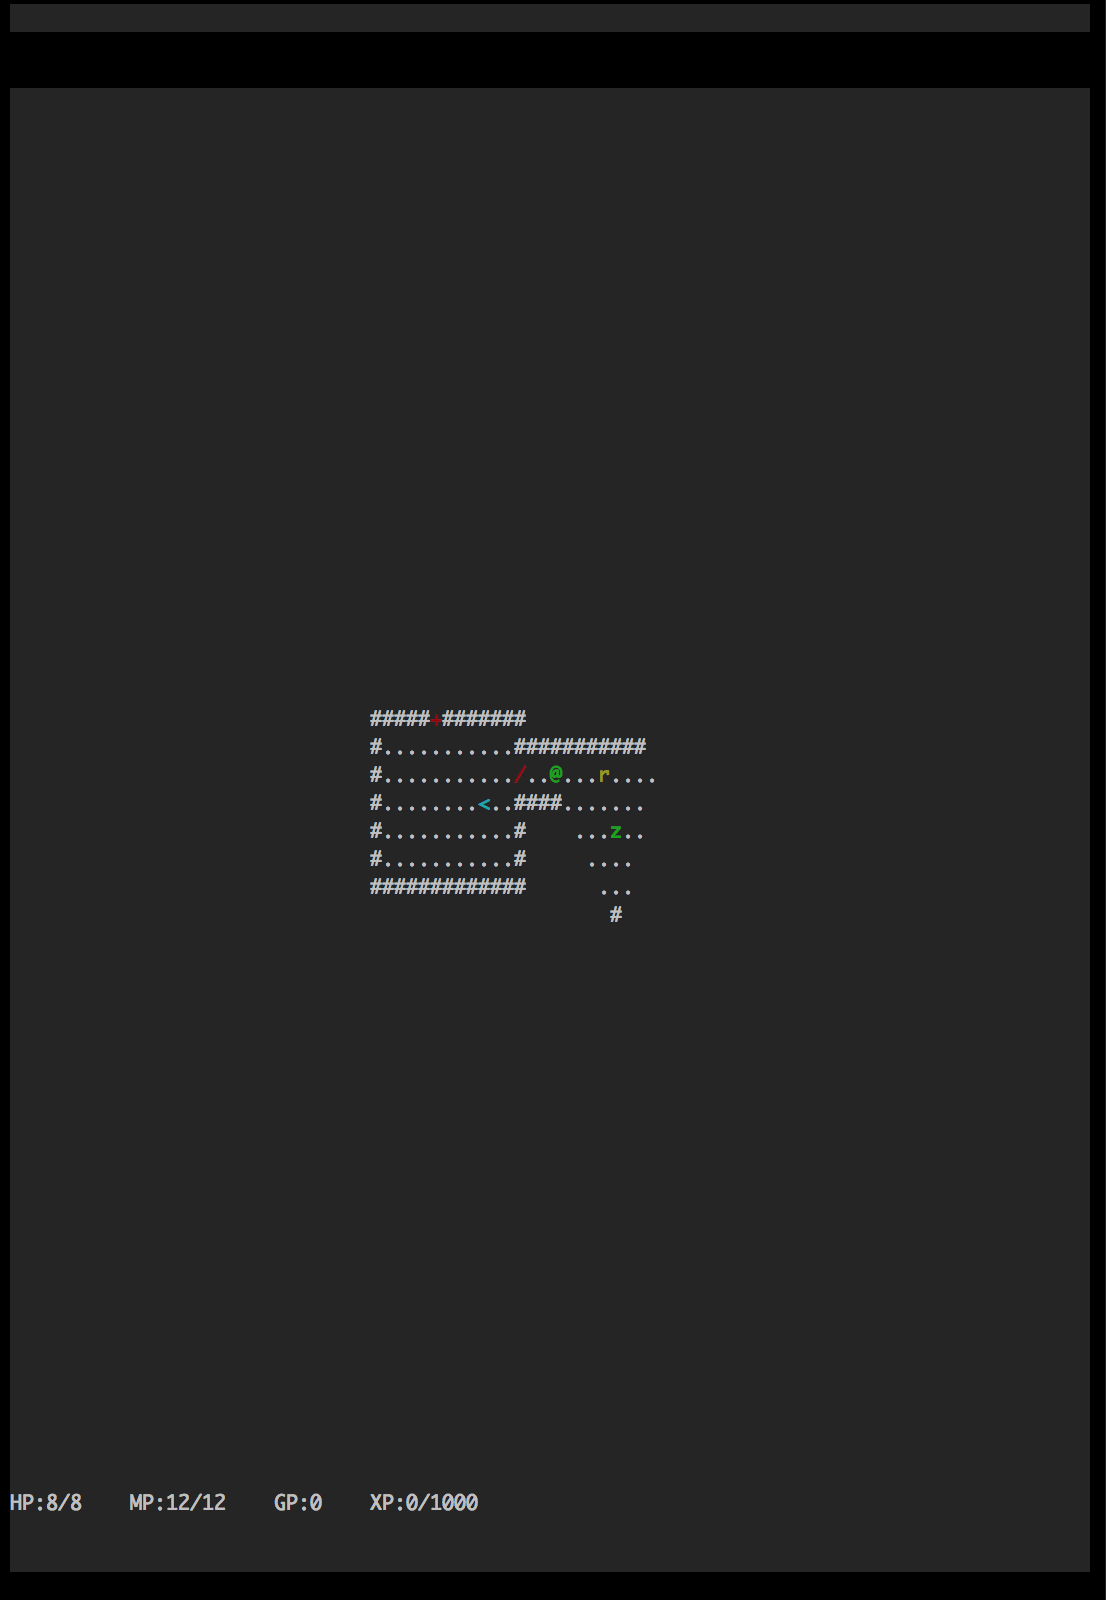
\includegraphics[width=17cm]{3.png}



\section{Useful links}
\begin{itemize}
  \item \href{https://www.debian.org/doc/manuals/debian-faq/ch-pkg_basics.en.html}{Basics of the Debian package management system}
  \item \href{https://en.wikipedia.org/wiki/RPM_Package_Manager}{RPM on wikipedia}
  \item \href{http://askubuntu.com/questions/453681/gcc-wont-link-with-m32}{askubuntu.com - gcc won't link with -m32}
\end{itemize}

\end{document}